% !TeX program = pdflatex
\documentclass[12pt,a4paper]{article}

\usepackage{iftex}
\ifPDFTeX
  \usepackage[utf8]{inputenc}
  \usepackage[T1]{fontenc}
\fi
\usepackage[italian]{babel}
\usepackage{libertine}
\usepackage[
  a4paper,
  left=2.5cm,
  right=2.5cm,
  top=2cm,
  bottom=3cm,
  footskip=1.35cm
]{geometry}

\usepackage{graphicx}
\usepackage{xcolor}
\usepackage{pagecolor}
\usepackage{titlesec}
\usepackage{fancyhdr}
\usepackage{enumitem}
\usepackage[colorlinks=true,urlcolor=cisfBlue,linkcolor=cisfBlue]{hyperref}

% Palette colori identica al PDF ufficiale approvato da EC
\definecolor{cisfBg}{RGB}{250,250,250}
\definecolor{cisfRed}{RGB}{153,0,0}
\definecolor{cisfBlue}{RGB}{0,51,153}

\pagecolor{cisfBg}

\setlength{\parindent}{0pt}
\setlength{\parskip}{8.2pt}

% Titoli di sezione centrati in rosso CISF
\titleformat{\section}
  {\centering\large\bfseries\color{cisfRed}}
  {}{0pt}{}
\titlespacing*{\section}{0pt}{15pt}{8pt}

% Footer istituzionale a 3 colonne su tutte le pagine
\pagestyle{fancy}
\fancyhf{}
\renewcommand{\headrulewidth}{0pt}
\renewcommand{\footrulewidth}{0pt}
\fancyfoot[L]{%
  {\footnotesize\color{cisfRed}%
  \shortstack[l]{%
    Conferenza Italiana Studenti di Fisica\\
    https://ai-sf.it/cisf27/\\
    cisf27@ai-sf.it%
  }}%
}
\fancyfoot[C]{%
  
\includegraphics[width=3.2cm]{logos/cisf27.png}%
}
\fancyfoot[R]{%
  {\footnotesize\color{cisfRed}%
  \shortstack[r]{%
    Coordinatori:\\
    francesco.isgro@ai-sf.it\\
    alessandro.dagostino@ai-sf.it%
  }}%
}

\begin{document}

% Intestazione prima pagina
\noindent
\begin{minipage}[c]{7.3cm}
  
\includegraphics[width=7.2cm]{logos/cisf27.png}
\end{minipage}%
\hspace{1.5cm}%
\begin{minipage}[c]{7.2cm}
  \textbf{Comitato Organizzatore CISF27}\\
  Conferenza Italiana Studenti di Fisica\\
  Associazione Italiana Studenti di Fisica\\
  Comitato Locale di Bologna\\
  \textit{Email:} \href{mailto:cisf27@ai-sf.it}{cisf27@ai-sf.it}\\
  \textit{Sito web:} \makebox[0pt][l]{\url{https://ai-sf.it/cisf27/}}
\end{minipage}

\vspace{14pt}

\section*{INFORMAZIONI GENERALI}

\textbf{CISF27} si terrà a \textbf{Bologna} dal \textbf{19 al 23 aprile 2027} e ospiterà \textbf{170 partecipanti}, a cui si aggiungeranno tutti i membri del Comitato Organizzatore e la persona che vincerà l'\textbf{open call della redazione di \textit{Fisicaffè}}, e che saranno così suddivisi: \textbf{150} avranno l'alloggio garantito dagli organizzatori presso il \textbf{Combo Bologna}, mentre i restanti \textbf{20}, a fronte di una \textbf{quota d'iscrizione minore}, potranno pernottare in una struttura di loro scelta in piena autonomia; per la persona che si aggiudicherà l'open call, il CO si impegna a garantire l'alloggio presso il \textbf{Combo Bologna}.

Le camere presso la struttura selezionata, tutte con bagno privato, saranno \textbf{quadruple (18)}, \textbf{triple (10)} e \textbf{doppie (24)} (alcune camere avranno letti matrimoniali e si potrà richiederli). Sarà possibile indicare le proprie preferenze in termini di tipologia di camera, genere di compagn* di stanza ed eventuali specifiche persone.

Il Comitato Organizzatore (CO) \textbf{si impegna ad accogliere ogni richiesta}, ma non esclude che per motivi logistici alcune preferenze possano non essere rispettate.

La Conferenza sarà \textbf{interamente tenuta in lingua italiana} e non saranno disponibili traduzioni: è necessario disporre di una buona conoscenza di essa. Inoltre, l'evento è destinato esclusivamente a \textbf{persone maggiorenni}.

Per partecipare alla Conferenza è \textbf{obbligatorio essere iscritt* ad AISF}: coloro che non sono iscritt* al momento dell'avvenuta selezione avranno l'obbligo di iscriversi pagando il \textbf{contributo associativo}, da aggiungersi alla quota di iscrizione a CISF27.

Le persone selezionate dovranno effettuare il \textbf{pagamento entro e non oltre una settimana} dalla comunicazione del Comitato Organizzatore. In caso di mancato pagamento, vi sarà \textbf{UN SOLO ripescaggio} ufficiale nei giorni successivi (le tempistiche saranno specificate in seguito agli/alle interessat*; se ogni persona selezionata versa la quota regolarmente non vi saranno ripescaggi). Ulteriori ripescaggi straordinari saranno eventualmente comunicati sui canali ufficiali di CISF27, ma non ne è garantita la presenza.

\section*{RIGETTO DELLA CANDIDATURA}

Il Comitato Organizzatore \textbf{rigetterà ogni candidatura}, automaticamente e irrevocabilmente, in cui:

\begin{itemize}[topsep=4pt,itemsep=4pt,parsep=0pt]
  \item la motivazione è creata con \textbf{chiaro ed evidente utilizzo di IA};
  \item è \textbf{dichiarato il falso};
  \item sono presenti \textbf{insulti, minacce, messaggi di odio di ogni tipo, messaggi di propaganda di ogni tipo, ingiurie} e in generale \textbf{ogni affermazione in contrasto con lo statuto di AISF e il codice etico adottato dal CO};
  \item il/la candidat* \textbf{non risulti iscritto ad AISF} entro i termini del pagamento.
\end{itemize}

\section*{CRITERI DI SELEZIONE}

Di seguito sono elencati i \textbf{criteri di selezione} che il Comitato Organizzatore applicherà laddove le richieste di partecipazione a CISF27 superino i posti disponibili.

\begin{enumerate}[topsep=5pt,itemsep=11pt,parsep=8pt]
  \item Passano \textbf{automaticamente} la selezione:
  \begin{itemize}[topsep=4pt,itemsep=4pt,parsep=0pt]
    \item i \textbf{membri del Comitato Organizzatore}, indicati nella sezione "Chi siamo" del sito ufficiale della Conferenza;
    \item i \textbf{membri del Comitato Esecutivo} (EC) di AISF;
    \item i \textbf{Presidenti dei Comitati Locali} (LC);
    \item 5 \textbf{membri della \textit{Commissione Fisicaffè}} che vengono indicati al CO da EC, in accordo con la Commissione stessa;
    \item la persona che vincerà l'\textbf{open call della redazione di \textit{Fisicaffè}}, che non dovrà pagare la quota d'iscrizione.
  \end{itemize}

  \item Ogni Comitato Locale avrà, indipendentemente dal proprio numero di membri e di candidature, una \textbf{quota minima di 5 partecipanti}, Presidente compres*. Qualora da un dato Comitato Locale pervenissero al CO meno di 5 canditature, saranno tutte accolte, a meno del rigetto di una o più di esse per le cause di cui sopra. Al \textbf{Comitato Locale di AISF Calabria} saranno riservati almeno \textbf{8 posti}, per supportare l'impegno dell'organizzazione di CISF28.

  \item Per assegnare i posti per ogni LC, uno dei criteri di maggiore importanza sarà la \textbf{proporzionalità rispetto al numero di candidature presentate}, pertanto si consiglia vivamente di incoraggiare ognun* nel proprio Dipartimento a consegnare la propria.

  \item Il Comitato Organizzatore si impegna a raggiungere la \textbf{parità di genere}.

  \item Possono partecipare studenti e studentesse di \textbf{Laurea Triennale}, \textbf{Laurea Magistrale} e \textbf{dottorandi}. L'evento non prevede partecipanti provenienti dalle scuole superiori.\\
  La distribuzione di partecipazioni \textbf{non sarà omogenea in funzione dell'età/anno di iscrizione ai corsi di laurea}: tenendo conto delle composizioni dei vari LC, delle partecipazioni alle scorse CISF, degli obiettivi associativi di EC e della linea adottata dal CO, verranno favorite alcune fasce di età rispetto ad altre, seppur non in maniera decisiva. Le candidature di esterni, cioè di persone non iscritte ad un CdL di Fisica/Astronomia/Scienze dei Materiali (e simili; si fa qui riferimento ai corsi di laurea sotto il Dipartimento di Fisica e Astronomia "Augusto Righi" di Bologna) o a un programma di dottorato saranno valutate caso per caso dal CO.

  \item Fattori di cui si terrà conto nelle candidature e motivazioni:
  \begin{itemize}[topsep=4pt,itemsep=4pt,parsep=0pt]
    \item \textbf{numero di partecipazioni} a CISF precedenti e ad altri eventi AISF;
    \item \textbf{partecipazione attiva nel proprio Comitato Locale}, nel Consiglio di Presidenza e nell'organizzazione di eventi locali e nazionali;
    \item disponibilità a \textbf{tenere una parallel session} o un \textbf{talk};
    \item \textbf{curiosità} nei vari aspetti della Conferenza;
    \item \textbf{entusiasmo} emerso nella motivazione (non è richiesto un esercizio di perfezione formale, ma un breve e partecipato racconto di sé).
  \end{itemize}
\end{enumerate}

\section*{AVVERTENZE}

A garanzia del processo di selezione, sarà possibile richiedere ulteriori informazioni sui criteri al CO e a EC che supervisionerà ogni passo.

Si prega di indicare nella candidatura la presenza di \textbf{allergie, intolleranze e preferenze alimentari}, così come \textbf{qualsiasi necessità fisica e logistica} che possa permettere al CO di rendere l'evento perfettamente inclusivo e accessibile a tutt*. \textbf{In nessun modo tali segnalazioni influiscono sulla selezione}.

La quota di iscrizione, una volta versata, \textbf{non è in nessun modo rimborsabile}. Ad ogni modo, il CO si offre comunque di fungere da intermediaro tra rinunciatar* e ripescat*

Restiamo a disposizione per ogni richiesta, domanda o chiarimento.\\
Vi ringraziamo per la vostra attenzione.

\vspace{6pt}

\begin{flushright}
  \begin{tabular}{@{}c@{}}
    Cordialmente,\\
    Francesco Isgrò - \textit{Coordinatore CISF27}\\
    Alessandro D'Agostino - \textit{Coordinatore CISF27}\\
    e tutto il \textit{Comitato Organizzatore}
  \end{tabular}
\end{flushright}

\vspace{14pt}

\noindent
\begin{minipage}[c]{6cm}
  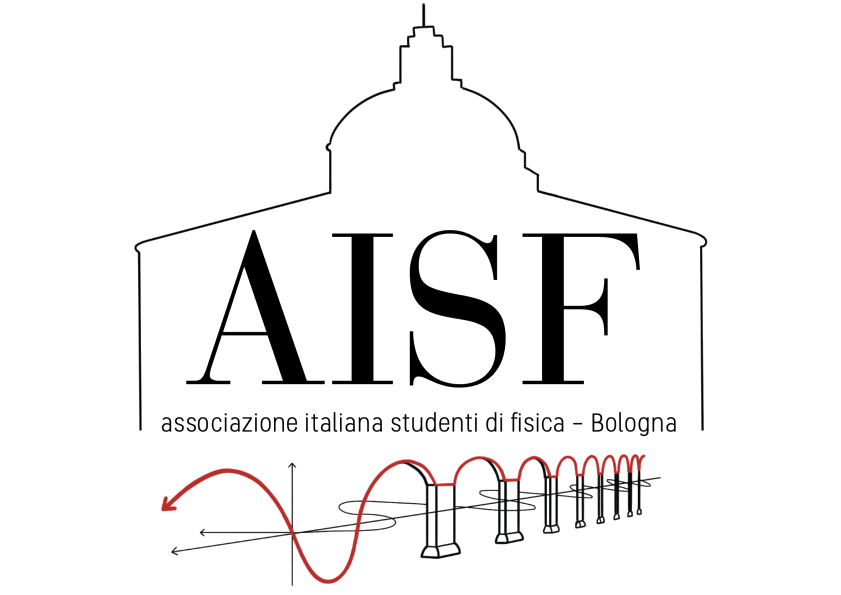
\includegraphics[width=6cm]{logos/aisf-bolo.png}
\end{minipage}%
\hfill
\begin{minipage}[c]{6cm}
  
\includegraphics[width=6cm]{logos/aisf.png}
\end{minipage}

\end{document}
